\documentclass[nonacm,acmtog]{acmart}
\usepackage{xcolor}
\usepackage{graphicx}
\usepackage{subcaption}
\newcommand{\todo}[1]{\textcolor{red}{\textbf{TODO}: #1}}
\newcommand{\TODO}{\textbf{\textcolor{red}{TODO}}}


% ==[ Header information ]======================================================
% Todo: Update document class file to typeset the author field like the subtitle

\title{CTAC-2019-2: Personal Tethers and the Extended Rappel}
\subtitle{The Mountaineers Climbing Technical Advisory Committee}

% ==[ Abstract ]================================================================

\begin{abstract}
   Extended rappels---where a climber's rappel device is attached to the
   harness via a short extension, rather than directly to the belay loop---are
   becoming an increasingly popular way to set up a rappel due to their
   advantages in both climber safety and comfort.  There are two primary ways
   the rappel extension can interact with the climber's personal tether: the
   tether and extension can either be combined into a single integrated system,
   or they can be kept separate as two independent systems.  This report looks
   at these two different options and evaluates each on their safety,
   efficiency, and ease-of-use.  We find that both alternatives meet the safety
   standard of CTAC and are acceptable rappel techniques for Basic climbers.
   However, based on its general popularity in climbing community and its
   increased efficiency in both setup time and gear, CTAC recommends using the
   integrated tether as the preferred setup in most cases.
\end{abstract}

\begin{document}
\maketitle

% ==[ Introduction ]============================================================

\section{Introduction}
\label{sec:intro}

   Once considered an advanced technique, the extended rappel has recently
   gained popularity in the climbing community and is now considered by many to
   be standard practice.  Extended rappels offer increased climber safety and
   comfort during a descent and have become a much more common sight at the
   crags and in the backcountry.  For the purposes of this report, an {\it
   extended rappel} is any rappel where the rappel device is connected to the
   climber's harness via a short extension---typically a Nylon or Dyneema
   sling---rather than attaching directly to the climber's belay loop.

   Though a full discussion of the advantages of extended rappels is beyond the
   scope of this report, CTAC has recommended this technique for use by
   climbers in the past \cite{mtnrs-rappel-blog1}.  Some of the arguments made
   in its favor in the previous recommendation include:

   \begin{itemize}
      \item The separation between autoblock backup and the rappel device
      enables smooth rappels while preventing the autoblock from jamming in the
      device.

      \item It enables multiple climbers to set up their rappels
      simultaneously, enabling more efficient descents for large
      groups~\cite{ctac:2019-3}.

      \item Since the autoblock backup is kept in-line with the device, the
      brake strands remain in the ideal braking position throughout the rappel.
   \end{itemize}

   There are two ways the extended rappel can be set up in conjunction with
   a climber's personal tether: either as an {\it integrated system}, or as
   {\it separated systems}.  In the integrated system, a single piece of
   webbing or other material is used as both the rappel extension and as the
   climber's tether to the anchor; in the separated system, the extension and
   tether are constructed from different pieces of material, creating two
   isolated systems that operate independently from one another.  The purpose
   of this report is to look at these two alternatives and evaluate each along
   a variety of axes, in order to determine to relative strengths and
   weaknesses of each.

   The rest of this report is organized as follows.  In \S\ref{sec:setup}, we
   describe how both the integrated and separated extensions are set up and
   describe how they can be used during a rappel; in \S\ref{sec:compare}, we
   look at both options and evaluate their strengths and weaknesses across a
   variety of axes; \S\ref{sec:discussion} offers a brief discussion of our
   findings; and \S\ref{sec:conclusions} concludes with our final
   recommendations on the use of these techniques.

% ==[ Setting Up the Systems]===================================================

\section{Setting Up the Systems}
\label{sec:setup}

   This section describes how to set up each type of extended rappel and
   briefly discusses how the extended rappels can be used by a climber during a
   descent.

\subsection{Integrated Tether and Extension}

   The integrated system is constructed with a single piece of material, which
   will serve as both the climber's personal tether and their rappel extension.
   Common options include improvised systems tied from a double-length nylon or
   Dyneema runner, or manufactured systems like the Metolius
   PAS~\cite{gear:pas} and the Sterling Chain
   Reactor~\cite{gear:chain-reactor}.  Each of these materials and products
   have their own strengths and weaknesses, though a full discussion of these
   is beyond the scope of the current report.  Interested readers are referred
   to \cite{ctac:2019-1} for more discussion on this topic.

   We'll describe below how to set up the integrated system with a
   double-length nylon runner, since this is one of the more common ways this
   system is used.  Details for setting up the system with the other types of
   leashes will be similar.

   \begin{enumerate}
      \item Attach the double-length runner to your harness by girth-hitching
      the runner to the hard-points of the harness
      (Figure~\ref{fig:int-step1}).  Position the sewn or tied part of the
      runner near your harness to prevent it from getting in the way later.

      \item Tie an overhand knot in the runner about halfway down its length.
      The position of the knot is important: it should be tied so that when the
      free end of the tether is clipped to the belay loop, the knot is furthest
      away from you, centered on the two legs (Figure~\ref{fig:int-step2}).

      \item Attach the rappel device to the runner with a locking carabiner by
      clipping in to the runner on both sides of the overhand knot tied in the
      previous step (Figure~\ref{fig:int-step3}).

      \item Attach an autoblock backup to the brake strands of the rappel, and
      clip it directly to the belay loop (Figure~\ref{fig:int-step4}).
   \end{enumerate}

   There are many other equivalent ways to set up the integrated system.  For
   example, another option is to tie an overhand-on-a-bight in the middle of
   the runner at step 2, instead of the simple inline overhand described above.
   This will create a ``master point'' that the rappel device can then be
   clipped to, rather than needing to clip around the knot.  However, the
   principles involved are identical and the discussions in \S\ref{sec:compare}
   and \S\ref{sec:discussion} apply to these alternatives as well.

   \begin{figure*}
      \centering
      \begin{subfigure}[t]{0.23\textwidth}
         \centering
         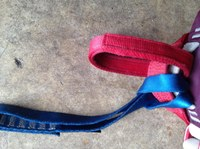
\includegraphics[width=0.95\textwidth]{images/int-step1.jpg}
         \caption{Girth hitch the runner to the harness' hard points.}
         \label{fig:int-step1}
      \end{subfigure}
      ~
      \begin{subfigure}[t]{0.23\textwidth}
         \centering
         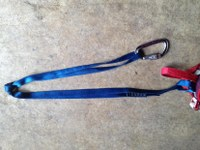
\includegraphics[width=0.95\textwidth]{images/int-step2.jpg}
         \caption{
            Tie an overhand knot in the runner about halfway down its length.}
         \label{fig:int-step2}
      \end{subfigure}
      ~
      \begin{subfigure}[t]{0.23\textwidth}
         \centering
         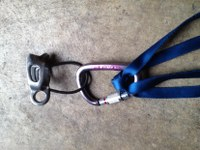
\includegraphics[width=0.95\textwidth]{images/int-step3.jpg}
         \caption{Clip the rappel device to both sides of the overhand knot.}
         \label{fig:int-step3}
      \end{subfigure}
      ~
      \begin{subfigure}[t]{0.23\textwidth}
         \centering
         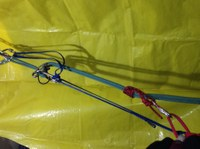
\includegraphics[width=0.95\textwidth]{images/int-step4.jpg}
         \caption{The autoblock attaches to the harness' belay loop.}
         \label{fig:int-step4}
      \end{subfigure}
      \caption{Setting up the integrated tether and rappel extension.}
   \end{figure*}

\subsection{Separated Tether and Extension}

   The separated system keeps the rappel extension and personal tether isolated
   from each other, and thus setting it up requires tying two components.  To
   create the separated system:

   \begin{enumerate}
      \item Attach a double-length nylon sling to your harness exactly as
      described in the first step of the integrated setup.

      \item Clip a locking carabiner to this double-length runner and secure it
      to the anchor.  This sling will be used as your personal tether.

      \item Basket hitch a single-length sling to the hardpoints on the harness
      and tie the ends together with an overhand knot, creating a single master
      point.  This sling will be used as the rappel extension.

      \item Connect the rappel device with a locking carabiner to the master
      point tied in the previous step.

      \item Attach an autoblock backup to the brake strands of the rappel and
      clip it to the belay loop, as before.
   \end{enumerate}

   See Figure~\ref{fig:separated} for an example of what the separated
   extension looks like when it is completed.

   \begin{figure}
      \centering
      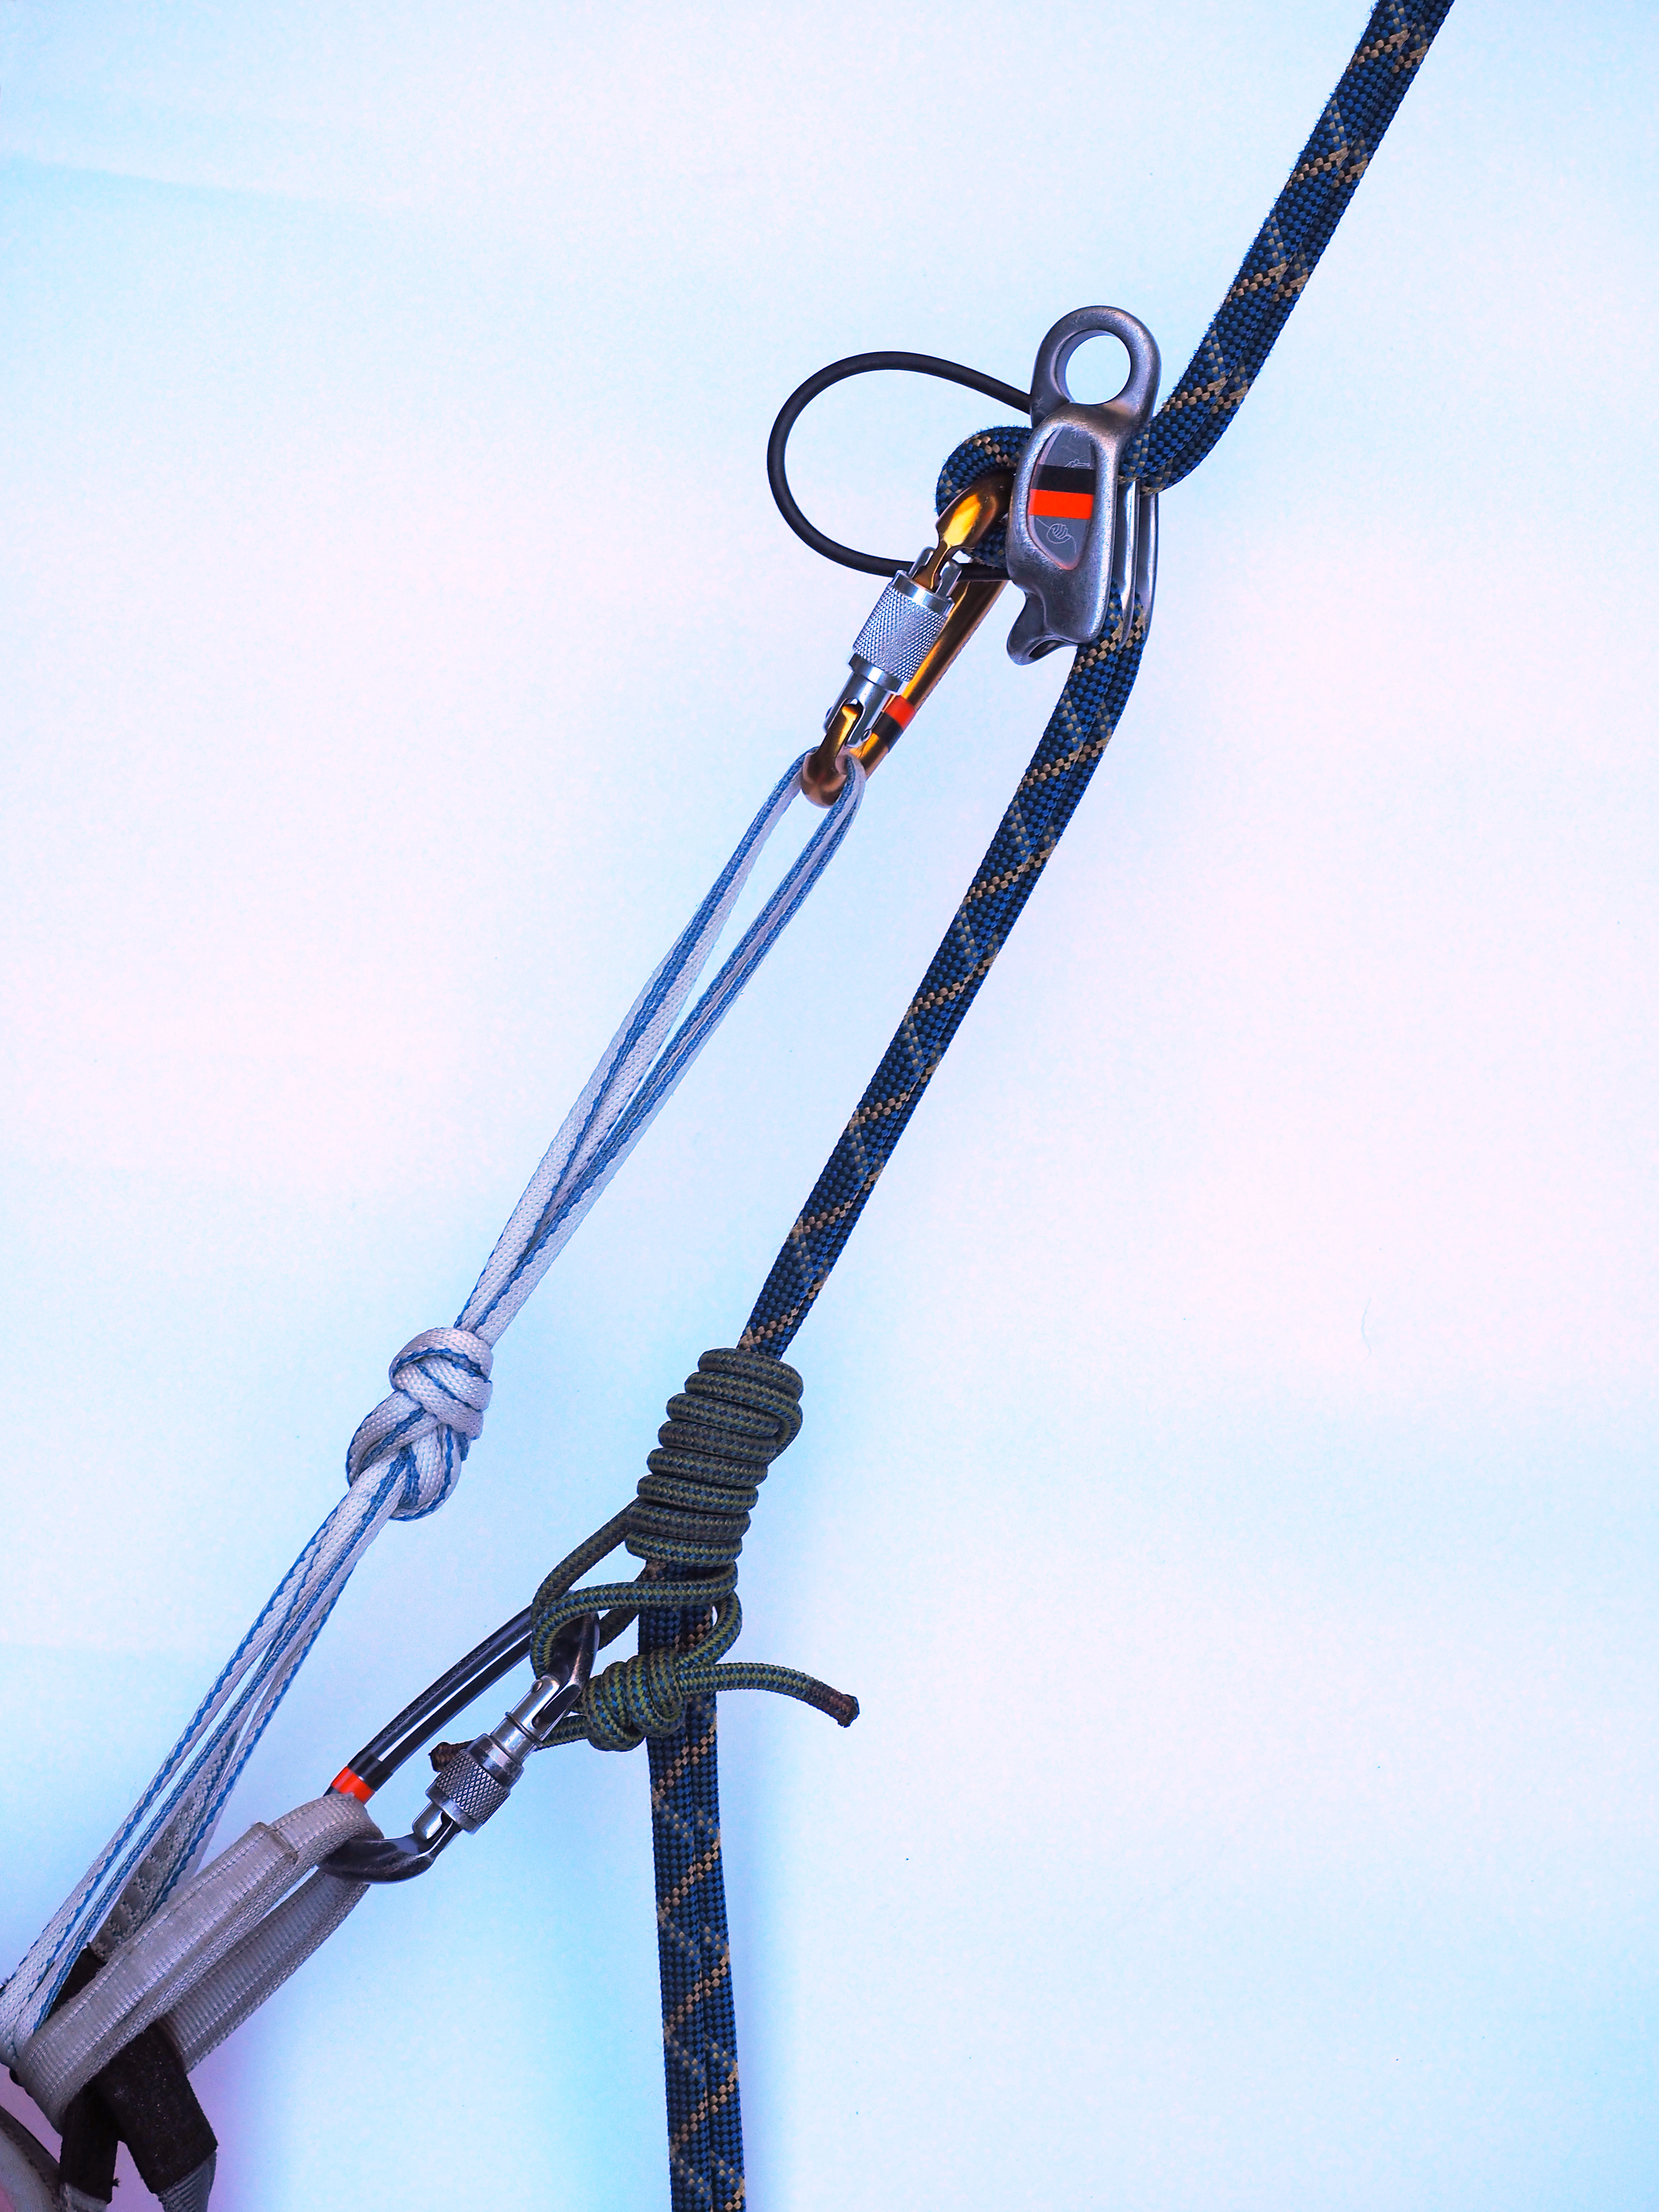
\includegraphics[width=0.25\textwidth]{images/separated.jpg}
      \caption{Example of the separated extension.  Tether isn't shown in this
         figure.}
      \label{fig:separated}
   \end{figure}

\subsection{Using the Extended Rappel}
\label{sec:using}

   Once set up, the process for using either of these systems while rappelling
   is nearly identical.  Begin by having your tether clipped to the anchor with
   a locking carabiner.  Then set the rope up for rappel as you normally would:
   pass the end of the rope through the rappel links, pull the rope through
   until its middle is at the anchor, and tie stopper knots on both ends of the
   ropes.

   Next, wrap an autoblock around the brake strands of the rope and clip it to
   the belay loop with a locking carabiner.  Pull a little slack through the
   autoblock, then pass a bight of both rope strands through your rappel device
   and clip it to the extension with a locking carabiner; the autoblock will
   hold the rope in place, making it easier to manage the rope in this step.
   In the integrated system, the rappel device will be clipped around the
   overhand knot on your sling, whereas in the separated system, it will be
   clipped to the master point of your dedicated rappel extension.

   Before trusting the system with live loads, it should first be tested to
   ensure it is set up correctly.  This can be done by pulling all excess slack
   through the rappel device and weighting it while keeping the tether attached
   to the anchor.  The autoblock should be allowed to hold the brake strands in
   place.  When set up correctly, the tether in either system will be slack,
   and the load will be held entirely by the rappel device and backup; this
   verifies the rappel and autoblock are both set up correctly.

   Once the system has been tested, it is ready to be used for descent.
   Establish a brake hand and remove the tether from the anchor, clipping it
   back to the belay loop.  Tend the autoblock throughout the descent.  When
   approaching the next rappel station, stop just above the anchor and clip
   the tether to the next anchor’s master point.  Continue the rappel until the
   tether is weighted and the rappel is slack.  The transfer to the next anchor
   is complete and the previous rappel can be removed.

   This process can be repeated for each pitch that needs to be descended.

% ==[Comparing the Techniques]==================================================

\section{Comparing the Techniques}
\label{sec:compare}

   Given that there are two different techniques to set up the extended rappel,
   when should one be used over the other?  That is the purpose of this
   section: to evaluate both techniques based on a variety of metrics,
   including the amount of gear required to set up, overall system complexity,
   the ability to test the rappel before committing, how difficult the system
   is to visually assess, and how common the technique is in the general
   climbing community.  Our goal is to highlight the strengths and weaknesses,
   if any, of each approach.

   A brief summary of our findings is included in Table~\ref{tab:side-by-side}.

   \begin{table*}
      \centering
      \begin{tabular}{|rp{2.25in}p{2.25in}|}
      \hline
         &
         {\bf Integrated System} &
         {\bf Separated System}  \\

      \hline
         {\bf Time and Gear Efficiency (\S\ref{sec:efficiency})} &
            Double-length sling, rappel device, autoblock, and 3 locking
               carabiners.  Uses one less sling and one less knot than the
               separated system.  Marginal advantage in this category.
               \vspace{0.1in} &
            Double-length sling, single-length sling, rappel device, autoblock,
               and 3 locking carabiners an autoblock.  Slightly less efficient
               than the integrated system. \\

         {\bf System Complexity (\S\ref{sec:complexity})} &
            Technically low; 7 points to visually assess.  Comparable to the
               separated sytem. &
            Technically low; 8 points to visually assess.  Comparable to the
               integrated system.
               \vspace{0.1in} \\

         {\bf Test before use? (\S\ref{sec:test})} &
            Yes. &
            Yes, as long as the tether is longer than the rappel extension.
            \vspace{0.1in} \\

         {\bf Commonly used? (\S\ref{sec:community})} &
            Well-known and widely used by recreational climbers.  Widely
               recommended by recognized climbing authorities. &
            Demonstrated in reputable sources, though not as widely published
               as the integrated system.  Also not as widely seen in the
               recreational climbing community.
               \vspace{0.1in} \\

         {\bf Rcmd. climber level (\S\ref{sec:discussion})} &
            Basic.  Simple knots and no complex mechanics; unlikely to set up
               incorrectly.  &
            Basic.  Simple knots and no complex mechanics; unlikely to set up
               incorrectly.
               \vspace{0.1in} \\

         {\bf Endorsed by CTAC? (\S\ref{sec:discussion})} &
            Yes. Preferred in most cases. &
            Yes. Acceptable alternative to the integrated system.
               \vspace{0.1in} \\
      \hline
   \end{tabular}
   \caption{Side-by-side comparison of the alternative methods for extended
      rappels}
   \label{tab:side-by-side}
   \end{table*}

\subsection{Time and Gear Efficiency}
\label{sec:efficiency}

   Efficiency in climbing systems is typically measured along two axes: by how
   long it takes to set the system up, and by how much technical gear is
   required.  In general, with all other things being equal, faster setups or
   those using less gear are preferred.

   Setting up the isolated system requires one double-length sling (acting as
   both the tether and the extension), a short loop of cord for the autoblock
   backup, the rappel device, and three locking carabiners (one each for the
   autoblock, the device, and the tether).

   Setting up the separated systems requires everything in the isolated setup,
   with the additional requirement of a second sling to be used as a dedicated
   extension.  And, though small, there is also an additional cost in time to
   tie and check this separate extension.

   In terms of time and gear requirements, the integrated system has a slight
   advantage over the separated systems, being both faster to set up and using
   one less sling.  However, the advantage is admittedly small, and by itself
   unlikely to be a strong motivating factor to advocate the use of the
   integrated system over the separated system.  For this report, the two are
   considered equal.

\subsection{System Complexity and Ease of Visual Assessment}
\label{sec:complexity}

   Another desirable attribute of a climbing system is that it  be easy to
   visually assess: the easier it is for climbers and their partners to verify
   the correctness of a system, the lower the likelihood of making a
   potentially life-threatening mistake.  As such, simpler systems should be
   preferred over more complex systems.

   %  Fortunately, both of the options
   %considered in this report are simple enough that any generally knowledgable
   %climber would be able to examine either one and have confidence in its
   %correctness, even when seeing it for the first
   %time.

   %This is especially true in the context of Mountaineers climbs, since teams
   %are often composed of climbers with widely varying backgrounds and levels of
   %experience.  Whenever possible, systems should be simple enough that any
   %generally knowledgeable climber would be able to examine it and have
   %confidence in its correctness, even when seeing it for the first time.
   %Fortunately, both of the options considered in this report meet this
   %criterion.

   In our comparison of the relative complexities of the two systems, we use
   the total number of points that need to be that need to be visually
   inspected for correctness once the system is set up to quantify the system’s
   complexity: more inspection points implies a more complex setup.

   Checking the integrated system requires the climber and their partner do the
   following:

   \begin{itemize}
      \item Verify the correct attachment of the tether to the hard points

      \item Ensure the gate of the carabiner used to clip the tether to the
      anchor is locked

      \item Inspect the attachment of the rappel device to the extension,
      making sure its clipped to both legs of the extension

      \item Verify the rappel device is set up correctly and the carabiner is
      locked

      \item Make sure the autoblock is correctly set up and clipped to the
      belay loop with a locked carabiner
   \end{itemize}

   This is a total of five things that need to be inspected for the integrated
   system.  For the separated system, all of the inspection points mentioned
   above still apply.  However, there's the additional requirement to inspect
   and verify that the dedicated extension sling is correctly tied and attached
   to the harness' hard points.

   Similar to the previous discussion of time and gear efficiency, the
   integrated option offers an ever-so-slight advantage in this category as
   well.  However, once again, that advantage is small and unlikely to be the
   sole factor for deciding to use one system versus the other.

\subsection{Ability to Test Before Use}
\label{sec:test}

   Any good rappel system should be testable before needing to completely
   commit to its use.  This helps catch errors in the rappel setup before they
   become potentially deadly mistakes.

   Both systems being examined in this report permit the climber to
   sufficiently test the setup before use, using the process described
   in \S\ref{sec:using}.  One note, however, is that when using the separated
   system, the tether must be longer than the rappel extension in order for
   this type of testing to be possible; otherwise it will be difficult to
   weight the extension without also weighting the tether, which limits the
   effectiveness of the test.  However, this is manageable and does not
   normally present difficulties in practice.

\subsection{Prevalence in the Climbing Community}
\label{sec:community}

   This category is more abstract than the others, but is considered by CTAC to
   be nearly as important as the rest.  Climbing systems require self checks
   and partner checks to validate their correctness.  Utilizing systems that
   are already widely recommended by recognized climbing authorities and the
   climbing public is highly desirable, since it becomes easier for climbers to
   find high-quality information and instruction in published resources, and a
   better chance your partner will recognize and properly assess the system
   being used.  Consistency with the current ``climbing norms'' should be
   preferred, with an understanding the what is considered ``normal'' now will
   undoubtedly evolve over time.

   From our own research, both techniques are well-known and taught by
   qualified climbing educators and guides as viable ways to set up an extended
   rappel.  We found, however, that the integrated option has a distinct
   advantage over the separated systems as being the more widely published
   option, both in online resources as well as published texts.  Though
   difficult to quantify empirically (as a complete survey of all published
   sources is not possible), a sampling of modern climbing references shows a
   number of sources that recommend its use, including
   \cite[pp.~213-214]{foth}, \cite[p.~25]{sr2}, \cite[pp.~219-220]{spi},
   \cite{vid:amga-ext-rap} and \cite{vid:siet-ext-rap}.  From a subjective
   perspective, it also appears to be the more common technique employed by
   climbers in the field based on the first-hand experiences of the authors of
   this report.

   The references that we found that teach the separated systems typically
   presented it as an alternative technique, after first demonstrating and
   recommending the integrated system \cite{vid:siet-ext-rap}.  Additionally,
   there were often qualifications to its use, such as those in
   \cite{fmg-extrap}, which presents it as an option that is ``best used for
   single pitch rappelling''.

   Based on our initial survey, it is our belief that the integrated rappel
   extension is and will continue to be the more widely used option in the
   field by recreational climbers, and thus has the advantage in this category.

   %\TODO: "This method creates a full strength extension with redundancy at
   %every part.  It is best used for single pitch rappelling as it does not have
   %a separate anchor extension and can be cumbersome to clip in during
   %multi-pitch descents." \cite{fmg- ext-rap}

   %* [[https://foxmountainguides.com/rappel-extension-options/]]
   %* [[https://www.youtube.com/watch?v=0qgygg8pzGI\&list=PLVPsXLzS-
   %CWE35A8kpIB4lcqNFg5zNRYc\&index=10]]

\subsection{General Comments}
\label{sec:general}

   When using the integrated tether and rappel extension, the length of the
   climber’s tether can limit their options for positioning themselves at a
   rappel station.  On crowded routes, this can lead to uncomfortable and
   cramped stances while waiting to descend.

   Although this crowding can often be prevented in the first place through
   efficient movement and transitions, sometimes it simply can’t avoided.  In
   these instances, keeping the extension separated from the tether may allow
   climbers to better position themselves while awaiting their turn to rappel.
   For instance, using a section of the climbing rope to secure yourselves to
   the anchor can offer versatile positioning and dynamic protection in the
   case of a fall.

\section{Discussion}
\label{sec:discussion}

   Based on our observations in the prior sections, we find that both
   alternatives are equally capable systems and use of either the integrated or
   separated rappel extensions on a Mountaineers climb should be considered a
   viable option.  Additionally, since neither technique involves anything more
   complicated than a few well-known knots and simple variations on standard
   practices, we believe the use of either of these systems is appropriate for
   Basic climbers.

   We note that in many cases the integrated systems has a number of marginal
   advantages over the separated systems.  Specifically, it requires less
   equipment (one less sling), it takes slightly less time to set up (only
   tying off a single sling, rather than two) and has fewer inspection points;
   it is also more widely documented and is, in our experience, a more commonly
   utilized method for extended rappels by the general public.  For these
   reasons we find the integrated option to be our preferred method for setting
   up an extended rappel in most cases.

   However, as discussed in \S\ref{sec:general} the separated option does have
   its advantages in some limited circumstances.  The example of being able to
   have a longer tether in the case of crowded belay stations might allow for
   more comfortable position of climbers awaiting their turn to descend.
   Although we generally would prefer to keep our stations less crowded (e.g.,
   through the use of more efficient systems and transitions), in some cases
   crowded stations can be unavoidable and the separated system with longer
   tethers are a viable management strategy.

\section{Conclusions}
\label{sec:conclusions}

   This report looked at two different methods of using a personal tether with
   an extended rappel: one where the tether and extension were integrated in a
   single system, and one where the two components were kept separate.  We
   compared the two approaches on a number of axes, including setup time, gear
   efficiency, system complexity, testability, and general acceptance within
   the climbing community.

   In practice, the benefits of an extended rappel can be leveraged effectively
   with either system and both alternatives are considered by CTAC to be safe
   options that can be recommended for use by Basic students.  However, we did
   find that the integrated option offers a number of small advantages to the
   separated systems---including reduced gear requirements, faster setup times,
   less complex visual assessments, and wider use in the general climbing
   community---that make it, in our opinion, the preferred technique for
   extended rappels in a majority of situations.

   %As such, both techniques are recommended for use by Basic climbers.  With
   %that in mind, The two systems are very similar and offer a lot of the same
   %advantages.    However, due to the slightly smaller gear requirements, and
   %smaller number of independent systems to check, the Committee recommends
   %using the integrated system as the preferred system, though the separted
   %systems can offer advantages in some scenarios.  \cite[ch.~1]{foth},
   %\cite{spi}, \cite{sr1}, \cite{mgm}.

   % Our report finds that both alternatives for constructing extended rappels
   % meet the safety standards of this Committee and are recommended for use by
   % Basic climbers.  However, for a number of reasons that will be discussed in
   % this report, the Committee %recommends the integrated system as the
   % preferred option in most scenarios, though the separated systems may be
   % better in certain circumstances.

\bibliographystyle{plain}
\bibliography{../ctac.bib}
\end{document}
